\chapter{Lexical Substitution}


\section{Probability in Context (PiC)}

\label{sec:pic}

\begin{figure}
\centering
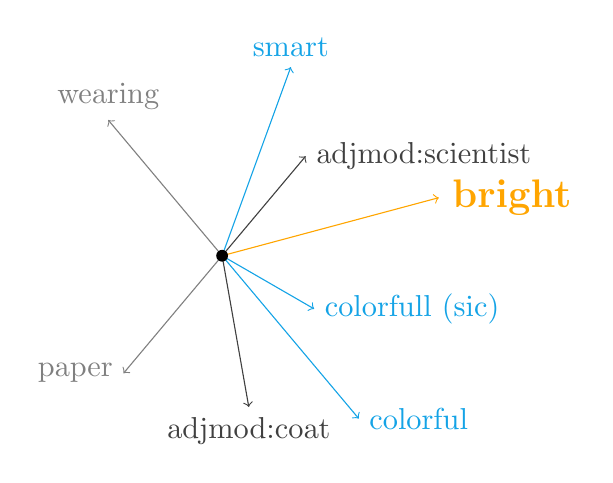
\begin{tikzpicture}[scale=1.5]
    \fontsize{11}{11}\selectfont
    \coordinate (origin) at (0,0);
    \draw [->,Gray] (origin) -- (130:1.5) node[above] {\word{wearing}};
    \draw [->,Gray] (origin) -- (230:1.3) node[left] {\word{paper}};
    \draw [->,Cerulean] (origin) -- (310:1.8) node[right] {\word{colorful}};
    \draw [->,Cerulean] (origin) -- (330:0.9) node[right] {\word{colorfull} (sic)};
    \draw [->,Cerulean] (origin) -- (70:1.7) node[above] {\word{smart}};
    \draw [->,darkgray] (origin) -- (280:1.3) node[below] {\word{adjmod\depinv:coat}};
    \draw [->,darkgray] (origin) -- (50:1.1) node[right] {\word{adjmod\depinv:scientist}};
    \fontsize{14}{14}\selectfont
    \draw [->,Orange] (origin) -- (15:1.9) node[right] {\bf{bright}};
    \fill (origin) circle (0.05);
\end{tikzpicture}
\caption{Cartoon illustration of how context vectors can disambiguate word senses.}
\label{fig:substitution}
\end{figure}

In this last section of our work, we switch over to our efforts on the Lexical
Substitution (LexSub) task. In the Lexical Substitution task, we are given
a sentence and target word, and must choose possible substitutes from the
entire vocabulary which preserve the meaning of the sentence.
As described in Section~\ref{sec:lexsub}, we view
LexSub as a proxy which captures a wide degree of lexical entailments {\em in
context}.

We propose a new measure, which extends
a previously successful, simple model to estimate the appropriateness of a
lexical substitute. As a introduction point for our measure, we review the work
of \newcite{melamud:2015:vsm}, which introduced several unsupervised measures
for word similarity in context: namely \balAddCos and \addCos. The main insight
of these unsupervised measures is the use of {\em context vectors}, related
to the insights discussed in Section~\ref{sec:lexmem}. Crucially, the models
of \newcite{melamud:2015:vsm} depend on syntactic context vectors, which
have been found more successful than just BoW measures in the literature
\cite{erk:2008:emnlp,dinu:2010:emnlp,thater:2010:acl,vandecruys:2011:emnlp}.
We note that these models are {\em not} the state of the art,
\cite{melamud:2015:naacl,melamud:2016:conll} but perform competitively while
remaining simple, extensible, and highly interpretable.

In the work of \newcite{melamud:2015:vsm} and others, substitutes are modeled
using a mixture of {\em out-of-context similarity} and {\em in-context
appropriateness}. The out-of-context similarity uses standard distributional
semantics cosine similarity (Equation~\ref{eq:cos}) in order to estimate how similar
the target is to the substitute, and remains fixed regardless of the sentential
context.  For this reason, this out-of-context (OOC) similarity is also used as
a baseline in the literature.

The in-context appropriateness attempts to directly model
whether a proposed substitute fits in the given sentential context. That is, if
one replaces the target with the substitute directly, would a reader still
consider this word {\em selectionally} agrees in the sentence. For example,
the in-context measures will give a low score for {\em dog purrs}, since dogs
usually do not purr.
To this end, it assumes the sentence is parsed, so that we have the full set of
syntactic neighbors of the target, $C$. Each of the context vectors
corresponding to elements of $C$ are then evaluated for their fit with the
proposed substitute, as illustrated in Figure~\ref{fig:syn}. For a given target
$t$, substitute $s$ and context $C$, the final \addCos~score is given as
\begin{equation}
  \text{addCos}(s|t,C) = \text{cosine}(s, t) + \sum_{c\in C} \text{cosine}(s, c).
\end{equation}
The model can be intuitively understood using the diagram in
Figure~\ref{fig:substitution}. For a given target ``bright,'' we will choose
the substitute (``smart'' or ``colorful'') which is {\em closer} to the
given context. If the context is ``scientist'' as in ``bright scientist,''
we will shift our prediction away from ``colorful'' and closer to ``smart,''
and vice versa for ``bright coat.'' This remains one of the simplest successful
models of Lexical Substitution to date. \newcite{melamud:2015:vsm} also consider
variants of this measure, including {\em balAddCos}, which equally
weights the out-of-context similarity with the in-context appropriateness:
\begin{equation}
  \text{balAddCos}(s|t,C) = \text{cosine}(s, t) + \frac{1}{|C|}\sum_{c\in C} \text{cosine}(s, c).
\end{equation}

In our work, we propose a new measure, called Probability-in-Context (PIC),\footnote{PIC is not strictly a probability measure; the name is a backronym for the purpose of the paper's title.}
which estimates the appropriateness of a substitute in a given context
\cite{roller:2016:naacl}.  Similar to \balAddCos, the measure has two
equally-weighted, independent components measuring the appropriateness of the
substitute for both the target and the context, each taking the form of a
softmax:
\begin{equation}
  \begin{aligned}
  \mbox{PIC}(s | t, C) &\propto P(s | t) \times P(s | C)\\
  P(s | t) &= \frac{1}{Z_t}\exp\left\{s^\top t\right\}\\
  P(s | C) &= \frac{1}{Z_C}\exp\left\{\sum_{c\in C}s^\top\left[Wc + b\right]\right\},
  \end{aligned}
  \label{eqn:pic}
\end{equation}
where the $Z_t$ and $Z_C$ are normalizing constants.
Our model differs from {\em balAddCos} in one major way: we base our similarity
estimates using the {\em unnormalized} inner product $s^\top t$ and $s^\top c$,
rather than normalized cosine similarities. We also introduce two additional
parameters, $W$ and $b$, which act as a simple linear transformation over the
original context vectors. These parameters are learned from the original
corpus, and serve only to tune how the fixed distributional vectors act in this
alternative objective function.

To identify the contribution of this parameterization versus the softmax
objective, we also introduce to a non-parameterized PIC ({\em nPIC}), which
does not contain the extra parameters:
\begin{equation}
  \begin{aligned}
  \mbox{nPIC}(s | t, C) &= P(s | t) \times P_n(s | C)\\
  P_n(s | C) &= \frac{1}{Z_n}\exp\left\{\sum_{c\in C}s^\top c\right\}
  \end{aligned}
  \label{eqn:npic}
\end{equation}

We compare our model to that of an out-of-context baseline (cosine) and the
{\em addCos} and {\em balAddCos} models of \newcite{melamud:2015:vsm}, which
outperformed other prior work at the time of its publication. We compare the
models on three data sets: SE07, the original LexSub data set
\cite{mccarthy:2007:semeval} which was explicitly developed to capture polysemy;
Coinco, a recent LexSub data set which contains substitutes for all content
words in a small corpus \cite{kremer:2014:eacl}; and TWSI2, which was developed
to be a large collection of lexical substitutes from a diverse corpus
\cite{biemann:2012:lrec}. We measure performance in Mean Precision@1, which
measures whether our best proposed substitute is contained within the set of gold
substitutes provided by annotators. In all models, we exclude any words sharing
the same lemma as the target, e.g. if the target is ``barking'' we do not
propose ``bark.''

\begin{table}
\begin{center}
\begin{tabular}{|l|r|r|r|}
  \hline
  {\bf Measure} & {\bf SE07} & {\bf Coinco} & {\bf TWSI2}\\
  \hline\hline
  %\multicolumn{4}{|c|}{Candidate Ranking (GAP)}\\
  %\hline
  %\ooc               &     44.2   &     44.5  &     57.9       \\
  %\addCos            &     51.2   &     46.3  &     62.2       \\
  %\balAddCos         &     49.6   &     46.5  &     61.3       \\
  %\hline
  %\ourmeas           &     51.3   &     46.4  &     61.8       \\
  %\ourmeasparam      & {\bf52.4}  & {\bf48.3} & {\bf62.8}      \\
  %\hline\hline
  %\multicolumn{4}{|c|}{All-Words Ranking (Mean Precision@1)}\\
  %\hline
  Cosine (OOC Baseline)                    &     11.7   &    10.9   &      9.8       \\
  addCos                                   &     12.9   &    10.5   &      7.9       \\
  balAddCos                                &     13.4   &    11.8   &      9.8       \\
  \hline
  nPic                                     &     17.3   &    16.3   &     11.1       \\
  PIC                                      & {\bf19.7}  &{\bf18.2}  & {\bf13.7}      \\
  \hline
  %\hline
  %\multicolumn{4}{|c|}{All-Words Ranking (Mean Precision@3)}\\
  %\hline
  %\ooc               &     9.7    &     8.6   &     7.0       \\
  %\addCos            &     9.0    &     7.9   &     6.1       \\
  %\balAddCos         &     9.8    &     9.1   &     7.4       \\
  %\hline
  %\ourmeas           &    13.1    &    12.1   &     7.9       \\
  %\ourmeasparam      &{\bf14.8}   &{\bf13.8}  &{\bf10.1}      \\
  %\hline
\end{tabular}
\end{center}
\caption{Lexical Substitution results for the all-words prediction task, measured
in Mean Precision@1.}
\label{tab:lexsub}
\end{table}

Table~\ref{tab:lexsub} contains results for all measures across all datasets.
We observe that PIC outperforms all other models by a significant
margin,\footnote{Wilcoxon signed-rank test, $p < 0.01$} including a relative
30\% improvement over \balAddCos in SE07 and Coinco. The nPIC also improves
substantially over the other baselines, indicating we gain benefit both from
the new objective function and the additional parameterization.  We next
strive to understand why both measures have a clear improvements over the
baseline models.

\begin{table*}[t]
  \begin{center}
  \begin{tabular}{|cccc|}
    \hline
    \ooc             & \balAddCos            & \ourmeas         & \ourmeasparam\\
    \hline\hline
    \multicolumn{4}{|c|}{You can sort of challenge them well, did you}\\
    \multicolumn{4}{|c|}{{\bf really} know the time when you said yes?}\\
    \hline\hline
    {    trully              } & {    proably             } & {    realy               } & {\bf actually            } \\
    {\bf actually            } & {    trully              } & {\bf truly               } & {\bf truly               } \\
    {    actaully            } & {    acutally            } & {\bf actually            } & {    already             } \\
    {    acutally            } & {    actaully            } & {    hardly              } & {    barely              } \\
    {    proably             } & {    probaly             } & {\bf definitely          } & {    just                } \\
    \hline
  \end{tabular}
  \end{center}
  \caption{Example where the \ourmeasparam~performs strictly better than other models. The target word and correct answers
  are bolded.}
  \label{tab:cherry}
\end{table*}

We characterize the models using a cherry-picked example,
given in Table~\ref{tab:cherry}. Although this example does not perfectly illustrate
the Lexical Substitution task, it does well at giving intuition as to why our
models perform better. We see that all four measures
tend to pick excellent substitutes which {\em semantically} agree with the
original target. However, the cosine and {\em balAddCos} models have a large number of
misspelled works in their list, while the nPIC and PIC measures contain
mostly correct spellings. This is because, somewhat surprisingly, the {\em
length} of the distributional vectors correlates strongly with the {\em
unigram} statistics of the word \cite{wilson:2015:arxiv}.
Therefore, by using the unnormalized inner
product, rather than cosine, our model naturally incorporates unigram priors,
allowing it to downweight rare, similar words. Indeed, a quantitative analysis
of the $W$ and $b$ parameters finds that they additionally exaggerate this
unigram bias \cite{roller:2016:naacl}.
Intuitively, it seems natural that unigram biases should hold a strong role in
Lexical Substitution, and that our model should wish to exploit this
information.

\section{Proposed: Lexical Substitution in RTE}

In Section~\ref{sec:lexsub}, we argued that Lexical Substitution is
related to textual entailment, partially standing
as a kind of in-context entailment. We have yet to provide any results
indicating that Lexical Substitution contributes in an
RTE system.  We propose that the Lexical Substitution model described in
Section~\ref{sec:pic} be used as additional features in the Lexical
Entailment classifier described in Section~\ref{sec:rtesubsystem}. Although we hope that
our Lexical Substitution model can positively contribute to the RTE pipeline,
we suspect improvements may be marginal.

The obvious way our Lexical Substitution model could contribute to the
task is by simply including the context-similarity features of the Lexical
Substitution model as another feature in the Lexical Entailment classifier.
That is, for a pair of words in the SICK dataset, measure the similarity of
their contexts using the $P(s|C)$ or $P_n(s|C)$ values proposed in
Equations~\ref{eqn:pic}~and~\ref{eqn:npic}. Although polysemy is not a
significant issue in the SICK dataset, we hope the additional information
about context will bolster predictions in borderline cases.

It may be necessary to find additional tricks in order to best integrate
this information into the lexical entailment classifier. For example, we
found the cosine binning trick described in Section~\ref{sec:rtesubsystem}
was necessary for getting distributional similarity to contribute. Similar
tricks, like binning or isolating the components of PIC, are likely
necessary in order to see any positive contribution.

Ultimately though, we suspect improvements to RTE  may be marginal, or even
negative, as polysemy is uncommon in the SICK dataset. We may need to analyze
differences in classification prediction, and which examples are {\em most}
affected by the LexSub features, in order to properly characterize contribution.


